\documentclass[]{article}
\usepackage{lmodern}
\usepackage{amssymb,amsmath}
\usepackage{ifxetex,ifluatex}
\usepackage{fixltx2e} % provides \textsubscript
\ifnum 0\ifxetex 1\fi\ifluatex 1\fi=0 % if pdftex
  \usepackage[T1]{fontenc}
  \usepackage[utf8]{inputenc}
\else % if luatex or xelatex
  \ifxetex
    \usepackage{mathspec}
  \else
    \usepackage{fontspec}
  \fi
  \defaultfontfeatures{Ligatures=TeX,Scale=MatchLowercase}
\fi
% use upquote if available, for straight quotes in verbatim environments
\IfFileExists{upquote.sty}{\usepackage{upquote}}{}
% use microtype if available
\IfFileExists{microtype.sty}{%
\usepackage{microtype}
\UseMicrotypeSet[protrusion]{basicmath} % disable protrusion for tt fonts
}{}
\usepackage[margin=1in]{geometry}
\usepackage{hyperref}
\hypersetup{unicode=true,
            pdftitle={Notes},
            pdfborder={0 0 0},
            breaklinks=true}
\urlstyle{same}  % don't use monospace font for urls
\usepackage{graphicx,grffile}
\makeatletter
\def\maxwidth{\ifdim\Gin@nat@width>\linewidth\linewidth\else\Gin@nat@width\fi}
\def\maxheight{\ifdim\Gin@nat@height>\textheight\textheight\else\Gin@nat@height\fi}
\makeatother
% Scale images if necessary, so that they will not overflow the page
% margins by default, and it is still possible to overwrite the defaults
% using explicit options in \includegraphics[width, height, ...]{}
\setkeys{Gin}{width=\maxwidth,height=\maxheight,keepaspectratio}
\IfFileExists{parskip.sty}{%
\usepackage{parskip}
}{% else
\setlength{\parindent}{0pt}
\setlength{\parskip}{6pt plus 2pt minus 1pt}
}
\setlength{\emergencystretch}{3em}  % prevent overfull lines
\providecommand{\tightlist}{%
  \setlength{\itemsep}{0pt}\setlength{\parskip}{0pt}}
\setcounter{secnumdepth}{0}
% Redefines (sub)paragraphs to behave more like sections
\ifx\paragraph\undefined\else
\let\oldparagraph\paragraph
\renewcommand{\paragraph}[1]{\oldparagraph{#1}\mbox{}}
\fi
\ifx\subparagraph\undefined\else
\let\oldsubparagraph\subparagraph
\renewcommand{\subparagraph}[1]{\oldsubparagraph{#1}\mbox{}}
\fi

%%% Use protect on footnotes to avoid problems with footnotes in titles
\let\rmarkdownfootnote\footnote%
\def\footnote{\protect\rmarkdownfootnote}

%%% Change title format to be more compact
\usepackage{titling}

% Create subtitle command for use in maketitle
\providecommand{\subtitle}[1]{
  \posttitle{
    \begin{center}\large#1\end{center}
    }
}

\setlength{\droptitle}{-2em}

  \title{Notes}
    \pretitle{\vspace{\droptitle}\centering\huge}
  \posttitle{\par}
    \author{}
    \preauthor{}\postauthor{}
    \date{}
    \predate{}\postdate{}
  

\begin{document}
\maketitle

\hypertarget{packrat}{%
\subsection{packrat}\label{packrat}}

Reproducible package manamement for R. Makes your R projects
reproducible by making them

\begin{itemize}
\tightlist
\item
  \textbf{isolated}: installing other packages won't break your project
\item
  \textbf{portable}: easy to share , even cross platform
\item
  \textbf{reproducible}: because it records the exact versions of the
  packages your project depends on
\end{itemize}

Each project has its own package library.

Funny story: so I've known about packrat for a few years now. I've known
what it does, and it made all the sense in the world. And yet I didn't
use it. God knows what my problem is, but it was only last month, when I
bought a new laptop, installed a new and different OS than my previous
one and wanted to start working on a project I was working on in the
spring, when it suddenly didn't work anymore. It was a big project with
dozens of interconnected files and several dozen packages, and it was
now broken. Now, I had already returned my old laptop to my employer so
I had no way of recreating the package environment that I had there. And
no easy way of figuring out which of the packages was the offending
package that had been updated in the meantime.

And it made me realise how incredibly lucky I had been that the
client---this was a consulting gig---the client was able to run the code
on their systems without any problems, presumably because theey had the
same outdated libraries installed as I had had on my old laptop. I was
terribly lucky, but I learned my lesson anyway. So from then on I use
packrat, actually preparing this talk was the first time I used it on a
new project.

But I wanted to bring up this story also to demonstrate that it is often
a slog, this reproducibility stuff. It's upfront work, and it's easy to
put it off. Although in the end it turned out that packrat is
ridiculously easy to setup, it is literally just one line of code, and
if you're initializing it on an existing large project you'll have time
to make yourself a quick cup of tea while it creates the snapshot of the
working library environment, but I was quite embarassed once I realised
I could have been doing this for years.. Instead I had to first have it
go wrong and have the code break, before I came to my senses and started
using this tool. It's normal, it's human. But it's also stupid. So don't
be stupid like I was, it's a lot less painful to get on the
reproduciblility bandwagon of your own accord than learning the hard
way.

(Hong et al. 2015)

\hypertarget{additional-details}{%
\subsection{additional details}\label{additional-details}}

In addition to software there are other environmental variables that
should be explicitly stated if they affect the results: " This
information may include: operating system, specific packages,
sub-routines, queries, files, libraries, scripts, service end-points,
configurations, parameters or workflows" "this information should be
described in the body of your paper, in the methods section, footnotes,
acknowledgements or appendices.

\begin{figure}

\includegraphics[width=0.7\linewidth,height=0.7\textheight]{/home/mz/Dropbox/XtraWork/teaching/2019-07-rep-res-humanities-oxford//figures/final-doc} \caption{PhD: final.doc [http://phdcomics.com/comics/archive.php?comicid=1531]}\label{fig:phd}
\end{figure}

\hypertarget{style-guide}{%
\subsection{style guide}\label{style-guide}}

\begin{figure}
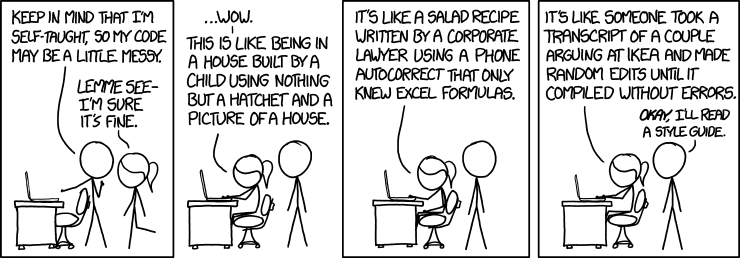
\includegraphics[width=0.9\linewidth]{/home/mz/Dropbox/XtraWork/teaching/2019-07-rep-res-humanities-oxford//figures/code_quality} \caption{[xkcd: Code Quality [https://xkcd.com/1513/]}\label{fig:xkcd}
\end{figure}

text

\hypertarget{references}{%
\section*{References}\label{references}}
\addcontentsline{toc}{section}{References}

\hypertarget{refs}{}
\leavevmode\hypertarget{ref-hong2015top}{}%
Hong, Neil P Chue, Tom Crick, Ian P Gent, Lars Kotthoff, and Kenji
Takeda. 2015. ``Top Tips to Make Your Research Irreproducible.''
\emph{arXiv Preprint arXiv:1504.00062}.


\end{document}
